\chapter{Einstieg --- Metrische Räume}

\section{Vorbemerkungen}

Inhalt dieser Vorlesung wird sowohl \emph{Stetigkeitsgeometrie} (Topologie) als auch \emph{metrische Geometrie} sein. Die unten abgebildeten Objekte sind im Sinne der Stetigkeitsgeometrie "topologisch äquivalent", im Sinne der metrischen Geometrie sind diese allerdings verschieden.

\begin{figure}[H]
  \label{img003-1}
  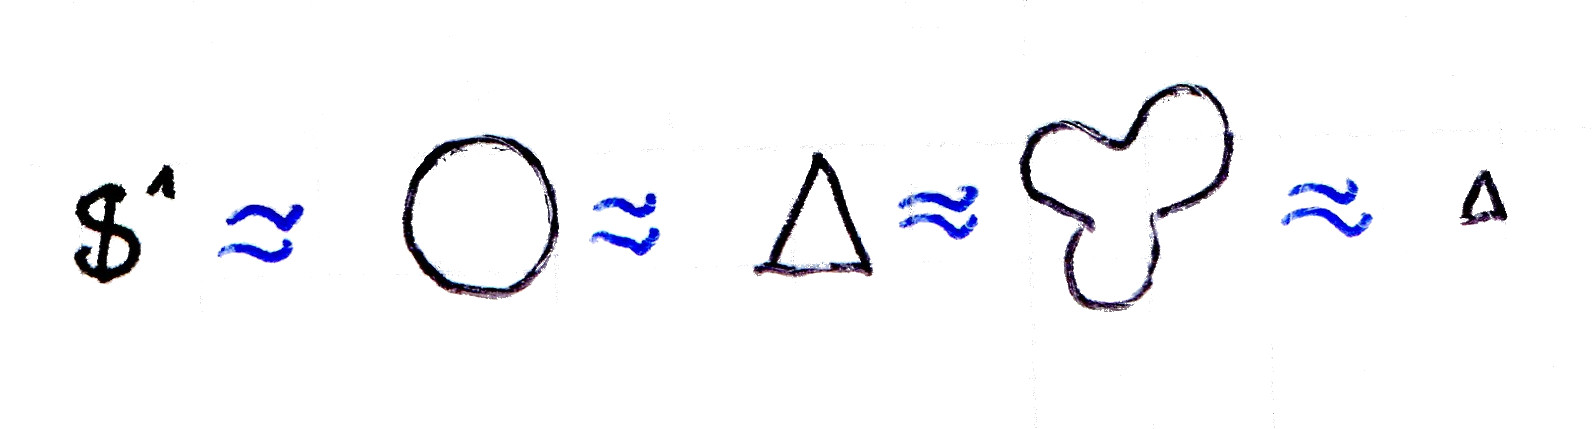
\includegraphics{img003-1}
  \caption{Diese Objekte sind topologisch äquivalent, metrisch allerdings nicht}
\end{figure}

\begin{remark}[Kartographieproblem]
  Ein zentrales Problem der Kartographie ist die \emph{längentreue} Abbildung einer Fläche auf der Weltkugel auf eine Fläche auf Papier. Mithilfe der Differentialgeometrie und der Gauß-Krümmung lässt sich zeigen, dass das nicht möglich ist.
\end{remark}

\section{Definitionen zu metrischen Räumen}

\begin{definition}[Metrik]
  \label{def:metrik}
  Sei $ X $ eine Menge. Eine Funktion $ d: X \times X \to \R_{\geq 0} $ ist eine \term{Metrik} (Abstandsfunktion), falls $ \forall x, y, z \in X $ gilt:
  \begin{enumerate}
    \item \textbf{Positivität}: $ d(x, y) = 0 \Leftrightarrow x = y $ 
    \item \textbf{Symmetrie}: $ d(x,y) = d(y,x) $
    \item \textbf{Dreiecksungleichung}: $ d(x,z) \leq d(x,y) + d(y,z) $
  \end{enumerate}
\end{definition}

\begin{definition}[Metrischer Raum]
  \label{def:metrischerRaum}
  Ein \term{metrischer Raum} ist ein Paar $ (X,d) $ aus einer Menge und einer \hyperref[def:metrik]{Metrik} auf dieser.
\end{definition}

\begin{definition}[Pseudometrik]
  \label{def:pseudometrik}
  Eine \term{Pseudometrik} erfüllt die gleichen Bedingungen wie eine \hyperref[def:metrik]{Metrik}, außer $ d(x,y) = 0 \Rightarrow x = y $ --- die Umkehrung gilt.
\end{definition}

\begin{definition}[Abgeschlossener $ r $-Ball um $ x $]
  \label{def:abgeschlossenerBall}
  Eine Teilmenge
  \begin{equation*}
    \overline{B_r(x)} \coloneqq \{ y \in X : d(x,y) \leq r \}
  \end{equation*}
  heißt \term{abgeschlossener $ r $-Ball um $ x $}.
\end{definition}

\begin{definition}[Abstandserhaltende Abbildung]
  \label{def:abstandserhaltendeAbbildung}
  Sind $ (X, d_X) $ und $ (Y, d_Y) $ \hyperref[def:metrischerRaum]{metrische Räume}, so heißt eine Abbildung $ f: X \to Y $ \term{abstandserhaltend}, falls
  \begin{equation*}
    \forall x, y \in X: d_Y(f(x), f(y)) = d_X(x, y)\text{.}
  \end{equation*}
\end{definition}

\begin{definition}[Isometrie] 
  \label{def:isometrie}
  Eine \term{Isometrie} ist eine bijektive \hyperref[def:abstandserhaltendeAbbildung]{abstandserhaltende Abbildung}. Falls eine Isometrie
  \begin{equation*}
    f: (X, d_X) \to (Y, d_Y)
  \end{equation*}
  existiert, so heißen $ X $ und $ Y $ \emph{isometrisch}.
\end{definition}

\section{Beispiele zu metrischen Räumen}

\begin{example}[Triviale Metrik]
  \label{bsp:trivialeMetrik}
  Menge $ X $,
  \begin{equation*}
    d(x, y) \coloneqq \begin{cases}
    0, &x = y \\
    1, & x \neq y
  \end{cases}\text{,}
  \end{equation*}
  also lässt mithilfe der \term{trivialen Metrik} jede Menge zu einem \hyperref[def:metrischerRaum]{metrischen Raum} verwursten. 
\end{example}

\begin{example}[Simple {\hyperref[def:metrik]{Metriken}}]
  \label{bsp:simpleMetriken}
  Sei $ X = \R $.\footnote{\textbf{Anmerkung}: Wenn $ d(x, y) $ eine \hyperref[def:metrik]{Metrik} ist, so ist auch $ \widetilde{d}(x, y) \coloneqq \lambda d(x, y) $ mit $ \lambda \in \R_{>0} $ eine Metrik.}
  \begin{itemize}
    \item $ d_1(s, t) \coloneqq |s-t| $ ist Metrik.
    \item $ d_2(s, t) \coloneqq \log(|s-t|+1) $ ist Metrik.
  \end{itemize}
\end{example}

\begin{example}[Euklidische Standardmetrik]
  \label{bsp:standardmetrik}
  $ X = \R^n $,
  \begin{equation*}
    d_e(x, y) \coloneqq \sqrt{\sum_{i=1}^n(x_i-y_i)^2} = \Vert x-y \Vert
  \end{equation*}
  ist die \term{(euklidische) Standardmetrik} auf dem $ \R^n $. Die Dreiecksungleichung folgt aus der Cauchy-Schwarz-Ungleichung\footnote{\textbf{Cauchy-Schwarz-Ungleichung}: $ \langle x, y \rangle \leq ||x||*||y|| \quad (x, y \in \R) $}.
\end{example}

\begin{remark}[aus LA II]
  \hyperref[def:isometrie]{Isometrien} von $ (\R^n, d_e) $ sind Translationen, Rotationen und Spiegelungen.
\end{remark}

\begin{example}[Maximumsmetrik]
  \label{bsp:maximumsmetrik}
  $ X = \R $,
  \begin{equation*}
    d(x, y) \coloneqq \underset{1 \leq i \leq n}{\max} \vert x_i-y_i \vert
  \end{equation*}
  ist \hyperref[def:metrik]{Metrik}.
\end{example}

\begin{example}[{\hyperref[bsp:standardmetrik]{Standardmetrik}} und {\hyperref[bsp:maximumsmetrik]{Maximumsmetrik}} allgemein: Norm]
  \label{bsp:norm}
  $ V $ sei $ \R $-Vektorraum. Eine \term{Norm} auf $ V $ ist eine Abbildung 
  \begin{equation*}
    \Vert\cdot\Vert : V \to \R_{>0}\text{,}
  \end{equation*}
  so dass $ \forall v, w \in V, \lambda \in \R $:
  \begin{enumerate}
    \item \textbf{Definitheit}: $ ||v|| = 0 \Leftrightarrow v = 0 $
    \item \textbf{absolute Homogenität}: $ ||\lambda v|| = |\lambda| * ||v|| $
    \item \textbf{Dreiecksungleichung}: $ ||v+w|| \leq ||v||+||w|| $
  \end{enumerate}
  Eine Norm definiert eine \hyperref[def:metrik]{Metrik} durch $ d(v, w) \coloneqq ||v-w|| $.
\end{example}

\begin{example}[Einheitssphäre]
  \label{bsp:einheitssphaere}
  \begin{equation*}
    S_1^n \coloneqq \{ x \in \R^{n+1} : ||x|| = 1 \}
  \end{equation*}
  ist die $ n $-te \term{Einheitssphäre}. \\
  Auf dieser ist mit
  \begin{equation*}
     d_W(x, y) \coloneqq \arccos(\langle x, y \rangle)
  \end{equation*}
  die \term{Winkel-Metrik} definiert.

  \begin{figure}[H]
    \label{img004-1}
    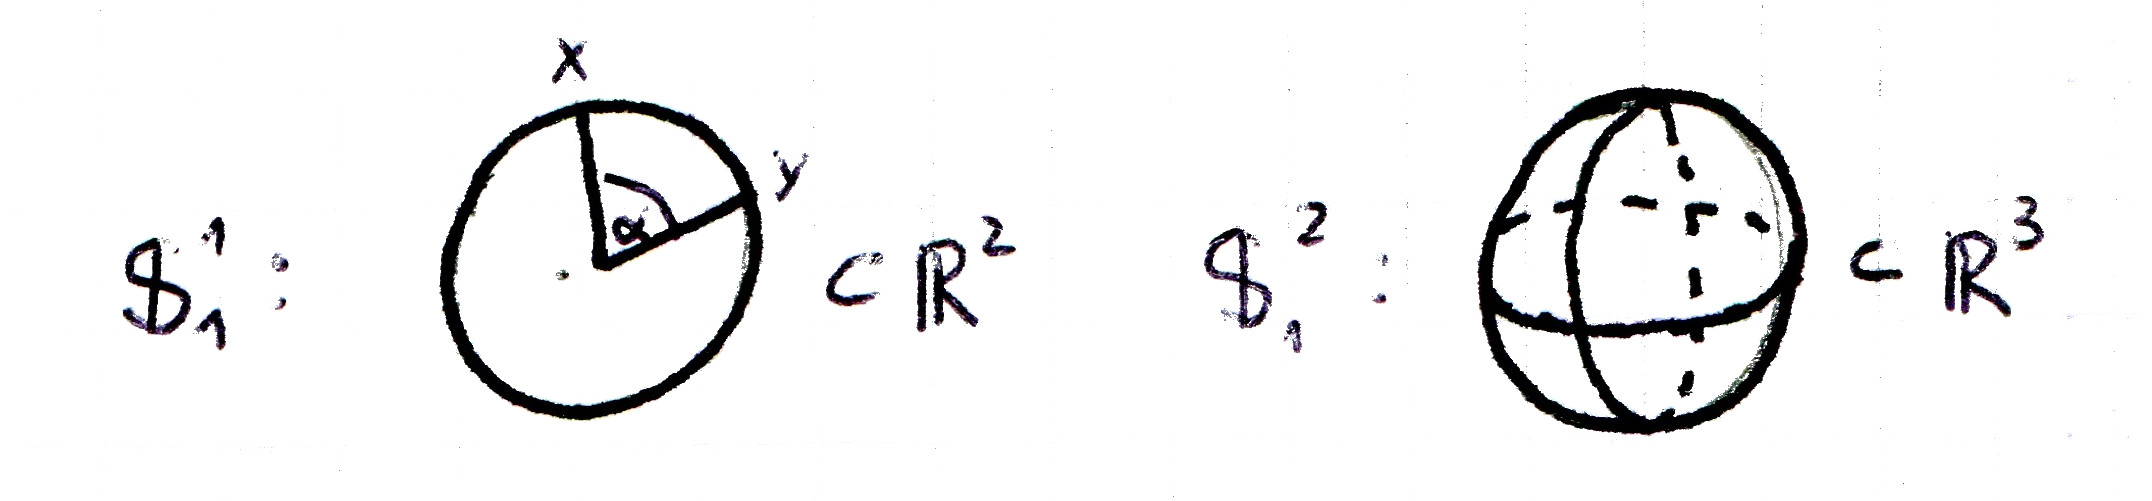
\includegraphics[width=.5\textwidth]{img004-1}
    \caption{Die erste und zweite Einheitssphäre}
  \end{figure}
\end{example}

\begin{example}(Hamming-Metrik)
  Es ist $ \mathbb{F}_2 $ der Körper mit zwei Elementen $ \{ 0, 1 \} $,
  \begin{equation*}
    X \coloneqq \mathbb{F}_2^n = \{ (f_1, \dots, f_n) : f_i = 0 \vee f_i = 1 \ (i \in {1, \dots, n}) \}
  \end{equation*}
  die Menge der binären Zahlenfolgen der Länge $ n $. Die \term{Hamming-Metrik} ist definiert als
  \begin{equation*}
    d_H: X \times X \to \R_{>0}, \quad d_H(u,v) = |\{ i : u_i \neq v_i \}|\text{.}
  \end{equation*}
\end{example}